% Explain how the CLI is implemented.
The \emph{CLI} is a very simple one, that has a separate thread for reading the input called input thread.
The input is read form the console constantly until the user hits enter.
Then the inputted line is sent to the main thread.
After that the thread waits for a response, the response is a boolean.
if the boolean is true then the program will stop, otherwise it start reading the console input again.
The thread repeats until it is stopped.


When the main thread receives a message from the input thread it tries to parse it into command.
The parser works by matching the first word in the input with the name of the commands.
If there is a match the commands specific parser is used to parse the rest of the input.
After a command is parsed it is then sent to the debug thread asynchronously.
It then waits for a response from the debug thread, when the response is received it prints it to the console.
After that is sends a response the the input thread.


An example of all the communication between the user and the threads can be seen in figure \ref{fig:cliflow}.
The example also shows what happens when a event is sent from the debug thread to the main thread.


\begin{figure}[h]
	\centering
	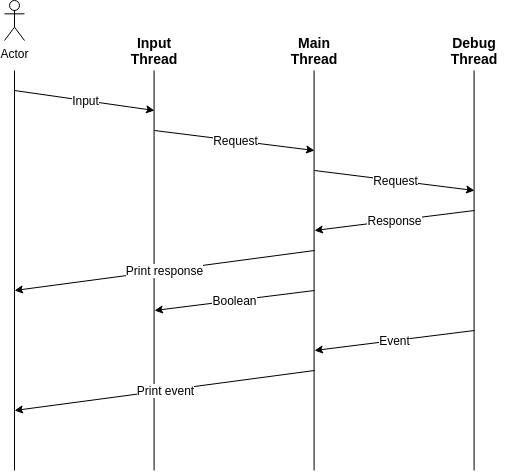
\includegraphics[width=0.9\textwidth]{cli_flow.png}
	\caption{A diagram showing the communication between the user/actor and the three different threads.}
	\label{fig:cliflow}
\end{figure}

